\newacronym{mimo}{MIMO}{\textit{Multiple Input Multiple Output}}
\newacronym{pid}{PID}{Proporcional Integral Derivativo}
\newacronym{mpc}{MPC}{Controle Preditivo Baseado em Modelo}
\newacronym{mhpc}{MHPC}{\textit{Model Heuristic Predictive Control}}
\newacronym{dmc}{DMC}{\textit{Dynamic Matrix Control}}
\newacronym{gpc}{GPC}{\textit{Generalized Predictive Controle}}
\chapter{Introdução}
\label{ch:introducao}

%Controle de processos é fundamental na industria.	[ok]
%Objetivo do controle.								[ok]
%Otimizar além de controlar.						[ok]
%Estratégias utilizando modelos matemáticos.		[ok]
%Porque não usar PID em alguns casos?				[ok - mais ou menos]
%Conceito do MPC.									[ok]
% (Brincalepe) Incluir histórico e maior detalhamento da importância do MPC atualmente      [ok]
% TODO: (Brincalepe) Incluir citações
O controle de processos tem fundamental importância no desenvolvimento industrial,
sendo amplamente utilizado em praticamente todos os segmentos da indústria,
contribuindo de maneira significativa para a maior velocidade na estabilização de sinais,
aumento da qualidade de produtos, diminuição de riscos e redução de custos operacionais.
Seu objetivo, de forma simplificada, consiste em avaliar e corrigir desvios entre um
valor desejado e o real valor medido na saída da planta para uma dada variável do
processo (ou variáveis, como em casos de processos com múltiplas entradas e múltiplas
saídas, também conhecidos por sua sigla em inglês \acrshort{mimo} (\textit{\acrlong{mimo}})).
A aplicação correta de estratégias de controle acarreta numa operação eficiente da
planta, mantendo suas variáveis relevantes em condições próximas às desejadas.
A sintonia bem-feita do controle auxilia também na otimização do processo,
possibilitando que o sistema opere com menor variabilidade, maximizando a produção
e minimizando a utilização de recursos. No \cref{ch:otimizacao} abordaremos mais
sobre otimização.
Modelos matemáticos podem auxiliar a estratégia de controle uma vez que um modelo da
planta ou processo pode ser utilizado para estabelecer a relação existente entre as
variáveis manipuladas e variáveis controladas, assim podendo auxiliar na predição do
comportamento dinâmico do sistema analisado. A modelagem matemática pode ser feita
utilizando dados empíricos ou através da aplicação de relações físico-químicas.

% TODO: (Brincalepe) Incluir citações
A estratégia de controle predominante na indústria é o controle \acrshort{pid}
(\acrlong{pid}) que, além de levar em consideração o efeito proporcional (P) do erro
medido, também atua em desvios relativos aos efeitos integrais (I) e derivativos (D).
Seu elevado número de aplicações deve-se a uma grande variedade de vantagens como:
sua rápida implementação, facilidade de compreensão, disponibilidade em praticamente
todas as plataformas industriais de controle e principalmente pelo fato de não requerer
um modelo matemático do processo; porém apesar de poder ser aplicado com eficiência em
uma grande variedade de processos, o controle \acrshort{pid} aparece com menos frequência
em sistemas não-lineares, como em plantas de controle de pH, por exemplo. Em casos como
esse, outra técnica bastante utilizada na indústria (porém em proporções bem menores
que o \acrshort{pid}) pode ser utilizada: o controle \acrshort{mpc} (\acrlong{mpc},
do inglês \textit{Model Predictive Control}). Uma introdução histórica desta técnica é apresentada
na seção a seguir e mais detalhes técnicos sobre ela serão apresentados no \cref{ch:mpc}.


% =====================================================================================================
% ============================================= Section ===============================================
% =====================================================================================================
\section{Introdução histórica ao \acrshort{mpc}}
\label{sec:intro_mpc}

Segundo \citeonline{Lee2011} em meados dos anos 50 as características essenciais do \acrshort{mpc}
já podiam ser observadas nas primeiras instalações de supervisórios de controle computadorizados,
porém, apesar de seus potenciais benefícios, esse tipo de controle não se difundiu muito
devido aos esforços necessário para mantê-lo e ao seu alto valor, até que aproximadamente
na metade dos anos 70 os microprocessadores e sistemas de controle distribuídos se tornassem
mais baratos e confiáveis. Não coincidentemente, por volta desta época começaram a surgir na indústria
e em seminários, publicações relatando a aplicação bem sucedida de controle baseado em modelo. \cite{Lee2011}

\citeonline{Lee2011} também relata que ainda durante os anos 70 a publicação das técnicas
\acrlong{mhpc} (\acrshort{mhpc} - Controle Preditivo Heurístico de Modelo) e
\acrlong{dmc} (\acrshort{dmc} - Controle Dinâmico de Matriz) mostrando grande sucesso prático,
impulsionaram o uso delas e de técnicas similares em refinarias de todo o mundo ocidental.
No geral os algorítmos por trás dessas técnicas apresentavam uma natureza heurística,
empregavam modelos baseados em resposta de domínio no tempo, eram completamente determinísticos
sem nenhum modelo explícito dos distúrbios, e não possuíam garantias de estabilidade nem
métodos para sintonia. Na mesma época, porém independente dos desenvolvimentos na indústria
de processos, surgia da comunidade de controle adaptativo o \acrshort{gpc} (Controle Preditivo
Generalizado, do inglês \acrlong{gpc}), que possuia motivações bem diferentes do \acrshort{dmc}:
o \acrshort{gpc} pretendia oferecer uma nova alternativa ao regulador de autoajuste, % TODO Adicionar footnote para self-tuning regulator
principalmente visando superar seu problema de robustez. Por causa disso ele aplicava problemas de controle
multivariável, porém carecia na inclusão de restrições, que era considerada uma característica
indispensável dos problemas de controle de processos.

Ao longo dos anos 80 os algorítmos \acrshort{mpc} se espalharam comercialmente a o embasamento
teórico da técnica começou a se consolidar. Nessa época muitas empresas (normalmente pequenas),
que ofereciam comercialmente soluções utilizando controle \acrshort{mpc}, foram adquiridas por
empresas maiores como a Aspen Tech e a Honeywell. No campo teórico aumentaram as discussões e
definições com relação a estabilidade, robustez e ao uso de modelos não-lineares. Além disso
os pesquisadores notaram que a utilização de modelos de espaço de estado poderia trazer mais
benefícios e juntamente com isso estabeleceram a forma padrão do algorítmo, demonstrada na
\cref{eq:mpc_standard_form}. \cite{Lee2011} 

\begin{equation}
	\label{eq:mpc_standard_form}
    \min_{\hat{u}(0),\cdots,\hat{u}(p-1)}
    \left\{
        V_p \triangleq \displaystyle\sum_{i=0}^{p-1}
            \left(\hat{x}^T(i)Q\hat{x}(i) + \hat{u}^T(i)R\hat{u}(i) \right)
            + \hat{x}^T(p)Q_t\hat{x}(p)
    \right\}
\end{equation}

\noindent
Sendo: 	\\
$ \hat{x}(i+1) = A\hat{x}(i) + B\hat{u}, \quad \hat{x}(0) = x_0 $

Ao longo das últimas décadas, desde o lançamento do \acrshort{dmc}, o \acrshort{mpc}
tem sido alvo de muito estudo teórico e prático, e passou de uma aplicação indústrial
heurística para uma das técnicas de controle mais influentes da atualidade \cite{Lee2011}.
Hoje podemos considerar o \acrshort{mpc}, segundo a definição de \citeonline{Seborg2011},
uma técnica de controle avançada para problemas de controle multivariável. Sendo que,
mesmo para um processo de múltiplas entradas e múltiplas saídas, onde existem restrições a
essas variáveis, é razoável assumir que possuindo o modelo dinâmico do processo e as medições
atuais do mesmo, pode-se predizer os valores de saída futuros, e então calcular as mudanças nos
valores de entrada baseando-se tanto nas previsões quanto no valor medido.

Após enormes avanços nas técnicas de resolução das equações aplicadas ao \acrshort{mpc},
atualmente seu uso não se limita mais à sistemas onde o tempo de resposta seja relativamente
lento, podendo então ser utilizado em diversas aplicações que eram consideradas impraticáveis
no passado. \citeonline{Lee2011} relata em seu artigo o uso do \acrshort{mpc} no controle
de tração de veículos, motorização automotiva, amortecimento de sistemas massa-mola magnéticamente
acionados, e muitos outros.


% =====================================================================================================
% ============================================= Section ===============================================
% =====================================================================================================
\section{Objetivos}
\label{sec:objetivos}

Este trabalho propõe, como objetivo principal, desenvolver um controlador \acrshort{mpc}
aplicado a um sistema didático com restrições de atuação.

Além disso os seguintes objetivos específicos também serão realizados:
\begin{itemize}
    \item Estudo do algorítmo do controle \acrshort{mpc}
    \item Avaliação o desempenho do controlador \acrshort{mpc} desenvolvido em
        comparação com um controlador \acrshort{pid}
    \item Comparação entre a implementação em duas ou mais plataformas,
        como MATLAB\textsuperscript{\tiny\textregistered}\footnote{
            MATLAB\textsuperscript{\tiny\textregistered} é uma plataforma                           % Footnote
            de programação projetada especificamente para engenheiros e cientistas                  % Footnote
            onde é possível desenvolver algoritmos, realizar a análise de dados,                    % Footnote
            criar modelos, aplicações, dentre outras coisas.},                                      % Footnote
        Python\footnote{
            Python é uma linguagem de programação de alto nível,                                    % Footnote
            interpretada e orientada a objeto, muito utilizada atualmente para                      % Footnote
            aplicações nas áreas de ciência de dados, aprendizagem de máquina,                      % Footnote
            identificação de sistemas, etc.}                                                        % Footnote
        ou similares.
\end{itemize}

% =====================================================================================================
% ============================================= Section ===============================================
% =====================================================================================================
\section{Motivação e justificativas}
\label{sec:motivacao_e_justificativas}

% TODO: (Brincalepe) Incluir citações
% TODO: (Brincalepe) Paragrafo muito longo. Quebrar em pedaços
Segundo \citeonline{Parkinson2018} o processo de determinar o melhor \textit{design}
para uma aplicação ou processo é chamado de otimização. Normalmente engenheiros
costumam tentar implementar tais técnicas em seus processos visando aumentar a
eficiência diminuindo os gastos, por exemplo projetando o menor trocador de calor
que realize a transferência de calor desejada, uma ponte de menor custo para o local,
ou mesmo maximizar o rendimento de um processo químico, porém, assim como nesses
exemplos, as variáveis e limitantes do processo podem ser inúmeras, fazendo com que a
tarefa de otimização se torne difícil caso o engenheiro utilize apenas uma combinação
de experiência, conhecimento, opiniões, etc. Para esses casos, ferramentas
computacionais de otimização são essenciais.

Dá-se o nome de Otimização Dinâmica ao processo de otimização que é realizado
dinamicamente ao longo do processo e, segundo \citeonline{Borrelli2017}, esta se
tornou uma ferramenta padrão na tomada de decisões numa grande variedade de áreas.
O controle \acrshort{mpc} é um modo de implementação da otimização dinâmica e a execução
deste trabalho em torno dessa técnica se deve ao fato de que ao longo dos últimos 25 anos
ela evoluiu para dominar a indústria de processos, onde tem sido utilizada em milhares
de problemas \cite{Borrelli2017}, bem como no controle dos processos de fabricação de cimento,
torres de destilação, plantas de PVC \cite{Camacho2007}, e também ao seu crescimento em outras
indústrias, como por exemplo a descrita por \citeonline{Yakub2013} em seu estudo comparativo
mostrando a utilização do \acrshort{mpc} no controle do sistema dinâmico de um automóvel.

% =====================================================================================================
% ============================================= Section ===============================================
% =====================================================================================================
\section{Organização do trabalho}
\label{sec:organizacao_do_trabalho}

% TODO: (Brincalepe) Descrever este trecho como sendo um objetivo específico
Este trabalho, além de visar abordar uma implementação prática de um controle \acrshort{mpc}
também busca ser um ponto de partida teórico e experimental para estudantes de graduação ou
pós-graduação, de língua portuguesa, que possuam algum conhecimento sobre teoria de controle,
porém que ainda estejam iniciando suas pesquisas sobre otimização de processos e controle preditivo.

A \cref{fig:estrutura_do_trabalho} indica um possível fluxo de leitura desde trabalho, sendo importante
ressaltar que os \cref{ch:otimizacao,ch:controle_preditivo} servem de base para uma melhor
compreensão do \cref{ch:mpc} e, portanto, podem ser lidos sem respeitar a ordem numérica dos mesmos.

\begin{figure}[h]
    \caption{Diagrama do fluxo de leitura do trabalho}
    \begin{center}
		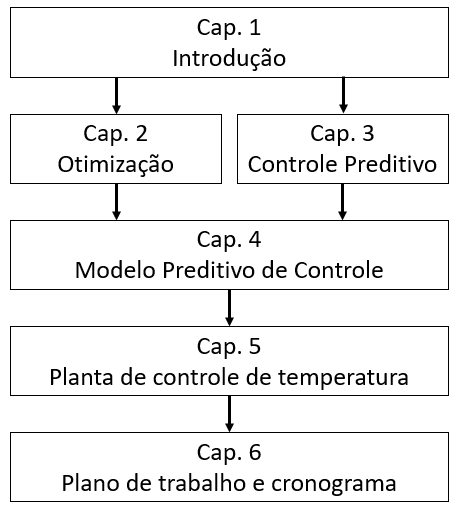
\includegraphics[width=0.4\textwidth]{./5_images/fig_estrutura_do_trabalho.png} 
		\label{fig:estrutura_do_trabalho}
    \end{center}
    \centering
    \makebox[\width]{Fonte: Autor}
\end{figure}